\chapter{Conclusiones y Trabajo futuro}
\label{chap:conclusiones}

En este capítulo se detallarán las conclusiones obtenidas del desarrollo de este proyecto, y se valorará si los objetivos propuestos en el capítulo \ref{chap:introduccion} han sido cumplidos. Además, se propondrán posibles líneas de trabajo futuro para mejorar este proyecto o que tomar como referencia para una posible segunda entrega.

\section{Conclusiones}

Este \acs{TFM} ha simulado el ciclo de desarrollo de un videojuego real en el que se ha implementado un videojuego completo con tecnologías \acs{VR}. Este desarrollo se ha dividido entregas, al final de las cuales se ha generado un entregable que se ha documentado a través de vídeos periódicos.

Tomando como referencia los resultados de la evaluación con usuarios reales realizada al final, se puede afirmar que se han cumplido los objetivos planteados al principio del proyecto; crear una experiencia inmersiva en la que el jugador se sintiera gratificado al resolver los diferentes acertijos que se le proponen. Además, esta experiencia puede motivarles para visitar museos reales. Por otro lado, si el usuario de \MineRVa padece algún tipo de impedimento físico que le impida hacerlo, se le ofrece una manera de emularlo haciendo uso del potencial motivador de un videojuego.

Por otro lado, con respecto a los objetivos secundarios, de índole más personal, se considera que este proyecto ha servido como primera toma de contacto tanto al desarrollo con tecnologías \acs{VR} y a sus principales frameworks y librerías como a los principales procesos y metodologías de desarrollo de videojuegos, así como al documento \acs{GDD} y las evaluaciones con usuarios.

Además, el trabajo de investigación realizado para el capítulo \ref{chap:estado_arte} ha servido para entender cómo han nacido las tecnologías utilizadas para desarrollar este proyecto y la motivación de sus creadores, como Blender o \acs{VRTK}, y todos problemas que tuvieron que superar para lograr sus objetivos.

Gracias a la división de trabajo al inicio del proyecto, la planificación por entregas y la utilización de metodologías ágiles ha sido posible terminarlo en el tiempo establecido, evitando así tener que realizar una fase de \textit{crunch} en la etapa final. Este término, que desafortunadamente está actualmente de moda, hace referencia al período en el que desarrolladores de un proyecto, normalmente informático, se ven obligados a trabajar por encima de las horas establecidas. Estos período suelen darse al final de los proyectos y se utilizan como única manera para poder llegar a la fecha de entrega estipulada. En su lugar, ha sido posible compaginarlo con el máster y las prácticas y completarlo a tiempo.

El desarrollo de este proyecto me ha permitido afianzar los conocimientos obtenidos a lo largo de las distintas asignaturas estudiadas en el máster, además de recordar conceptos aprendidos a lo largo de la carrera relacionados con interfaces y sistemas interactivos y de tiempo real.

En definitiva, considero que este proyecto es el principio de mi carrera profesional, que espero poder dedicar al desarrollo de sistemas interactivos y en la que espero poner en práctica los conocimientos adquiridos tras la realización de este \acs{TFM}.


\section{Trabajo futuro}

A pesar de haber completado todos los objetivos propuestos inicialmente y haber aportado algunos nuevos a lo largo del desarrollo, hay algunas opciones que no se han llevado a cabo o bien por falta de tiempo o bien porque no se cree que actualmente aporten suficiente valor al producto en comparación con su carga de trabajo.

Además, a diferencia de otro tipo de proyectos informáticos, los videojuegos son especialmente susceptibles a, en lugar de mejorar una versión, reunir todas estas mejoras y desarrollar una nueva entrega, teóricamente mejor que la anterior, por lo que es especialmente interesante plantear un posible trabajo futuro en proyectos de esta naturaleza. 

A continuación se presentan las líneas de trabajo futuro más relevantes que podrían seguirse de este proyecto.

\begin{itemize}
    \item \textbf{Traducir a diferentes idiomas.} Uno de los objetivos de un videojuego es que sea jugado por el mayor número de personas posibles, y una de las mayores barreras de entrada, si no la que más, es el lenguaje. 
    
    Por ello, se ha añadido el esqueleto de lo que en un futuro podría ser el soporte multilenguaje. Para lograr esto, se ha añadido un selector en los script de gestión de los diálogos y las descripciones de los cuadros en el que se puede seleccionar un lenguaje, que por debajo simplemente de qué carpeta leer los archivos de texto. En la figura \ref{fig:languaje-selector} puede verse el caso de este último, que actualmente solo soporta el español.

    \begin{figure}[!h]
    \begin{center}
    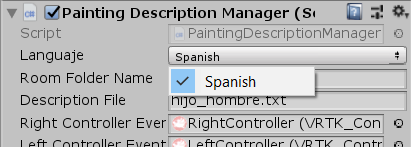
\includegraphics[width=0.6\textwidth]{imagenes/8/languaje-selector.png}
    \caption{Script para cambiar el idioma desde el inspector}
    \label{fig:languaje-selector}
    \end{center}
    \end{figure}

    Siguiendo este enfoque, cada lenguaje tendría una carpeta dentro del directorio de diálogos y descripciones. Para completarlo, en el menú principal sería necesario incluir una sección desde la que el usuario pudiera seleccionar su lenguaje, y ésto actualizase el resto de scripts.
    
    De este modo sería suficiente con proporcionar a un traductor los archivos de texto del juego e incluirlos directamente dentro de su carpeta, una vez traducidos, sin necesidad de modificar el código fuente. Además, sería posible que las traducciones de los diálogos se dividieran en un número mayor o menor de archivos, ya que el sistema continua leyéndolos hasta que no encuentra más, lo que les proporcionaría mayor flexibilidad y les permitiría a los traductores adaptar estas traducciones de mejor manera.

    \item \textbf{Guardar y cargar partidas.} Quizá uno de las mayores ausencias de funcionalidad del juego es la habilidad para poder guardar la partida y poder continuarla en un futuro. Esto no ha sido una prioridad a lo largo del desarrollo por varios motivos, siendo el principal que en un juego relativamente corto (si tomamos como referencia el vídeo mostrando el juego terminado, aproximadamente media hora) y que la dificultad de una sala reside en saber qué hay que hacer para avanzar, y una vez que se ha completado es inmediato, se considera que no es algo esencial y que el su lugar se podría añadir en un futuro.
    
    Además, por la naturaleza del juego sería relativamente sencillo guardar una partida en disco, bastando simplemente con almacenar la sala en la que se quedó el jugador, lo que si quisiéramos simplificar aún más podría traducirse en un selector de salas en el menú principal.
    
    \item \textbf{Aumentar la rejugabilidad.} Como ya ha podido verse en el punto anterior y en los resultados de las evaluaciones con usuarios, el principal problema del juego es su falta de rejugabilidad; esto es, una vez que el usuario completa el juego y conoce la historia y las salas y sus pruebas no tiene ninguna motivación por volver a jugar. 
    
    Esto podría intentar evitarse sin desviarse excesivamente de la naturaleza del juego variando, por ejemplo, los cuadros que hay en cada sala. Sería algo relativamente sencillo, y simplemente sería necesario elegir aleatoriamente qué cuadros va a tener una sala en el momento de cargarla. No sería una generación procedural completa, ya que la sala en sí sería la misma siempre; simplemente se sustituirían unos cuadros por otros que habrían sido modelados e incluidos previamente.
    
    \item \textbf{Publicación.} El paso lógico de un videojuego terminado es ser publicado, ya sea gratuito o de pago, y la plataforma en la que lo hacen la mayoría de los juegos es Steam, aunque por cuestión de agenda no ha sido posible hacerlo. Aún así, la versión compilada del juego está disponible públicamente en la sección \textit{releases} del repositorio del proyecto o, de manera equivalente, siguiendo el siguiente enlace.
    
    \begin{center}
        \url{https://github.com/gomezportillo/mineRVa/releases}
    \end{center}
    
\end{itemize}


